\documentclass[11pt,a4paper]{article}

\usepackage[T1]{fontenc}
\usepackage[utf8]{inputenc}
\usepackage{lmodern}
\usepackage{microtype}
\usepackage{geometry}
\geometry{left=23mm,right=23mm,top=22mm,bottom=24mm,headheight=22pt}
\usepackage{setspace}
\setstretch{1.06}
\usepackage{amsmath,amssymb,mathtools,bm}
\usepackage{array,tabularx,booktabs}
\usepackage{enumitem}
\usepackage{xcolor}
\usepackage[most]{tcolorbox}
\usepackage{tikz}
\usetikzlibrary{arrows.meta,calc}
\usepackage{needspace}
\usepackage{etoolbox}
\usepackage{fancyhdr}
\usepackage{titlesec}
\usepackage[hidelinks]{hyperref}

\definecolor{ink}{HTML}{414141}
\definecolor{vuBurgundy}{HTML}{78003F}
\definecolor{vuPink}{HTML}{E64164}
\definecolor{vuDarkGray}{HTML}{414141}
\definecolor{vuLightGray}{HTML}{DCDCDC}
\definecolor{navy}{HTML}{123653}
\definecolor{blue}{HTML}{174F78}
\definecolor{paleBlue}{HTML}{F1F6F9}
\definecolor{paleBurgundy}{HTML}{FAF2F6}
\definecolor{palePink}{HTML}{FDF3F5}
\definecolor{workGray}{HTML}{ABB3BB}
\definecolor{softGray}{HTML}{F5F5F5}

\color{ink}
\setlength{\parindent}{0pt}
\setlength{\parskip}{0.55em}
\clubpenalty=10000
\widowpenalty=10000
\displaywidowpenalty=10000
\setlist[itemize]{leftmargin=1.5em,itemsep=0.25em,topsep=0.25em}
\setlist[enumerate]{leftmargin=1.8em,itemsep=0.25em,topsep=0.25em}
\setcounter{tocdepth}{2}
\setcounter{secnumdepth}{2}

\titleformat{\section}
  {\Large\bfseries\color{vuBurgundy}}{\thesection}{0.65em}{}
\titleformat{\subsection}
  {\large\bfseries\color{blue}}{\thesubsection}{0.65em}{}
\titlespacing*{\section}{0pt}{1.6em}{0.65em}
\titlespacing*{\subsection}{0pt}{1.2em}{0.45em}
\pretocmd{\section}{\Needspace{8\baselineskip}}{}{}
\pretocmd{\subsection}{\Needspace{5\baselineskip}}{}{}

\pagestyle{fancy}
\fancyhf{}
\fancyhead[L]{\small\color{vuBurgundy}\textbf{Special Relativity I}}
\fancyhead[R]{\small\color{ink!65}Lecture notes}
\fancyfoot[C]{\small\color{vuBurgundy}\thepage}
\renewcommand{\headrulewidth}{0.4pt}
\renewcommand{\headrule}{\hbox to\headwidth{%
  \color{vuBurgundy}\leaders\hrule height \headrulewidth\hfill}%
  \vskip-\headrulewidth}

\hypersetup{
  pdftitle={Special Relativity I - Lecture Notes},
  pdfsubject={Cosmology lecture notes with proof and derivation spaces},
  colorlinks=true,
  linkcolor=navy,
  urlcolor=blue
}

\newcommand{\vect}[1]{\bm{#1}}
\newcommand{\dd}{\mathrm{d}}
\newcommand{\R}{\mathbb{R}}
\newcommand{\id}{\mathbf{I}}
\newcommand{\transpose}{\mathsf{T}}
\newcommand{\order}[1]{\mathcal{O}\!\left(#1\right)}

\newcommand{\slideref}[1]{%
  \par\smallskip
  {\footnotesize\color{ink!60}\textsc{Source slide #1}}\par
}

\newtcbtheorem[number within=section]{definition}{Definition}{
  enhanced,colback=paleBlue,colframe=blue,
  colbacktitle=blue,coltitle=white,fonttitle=\bfseries,
  boxrule=0.7pt,arc=1.4mm,
  left=2.5mm,right=2.5mm,top=1.7mm,bottom=1.7mm
}{def}

\newtcbtheorem[use counter from=definition]{postulate}{Postulate}{
  enhanced,colback=paleBlue,colframe=blue,
  colbacktitle=blue,coltitle=white,fonttitle=\bfseries,
  boxrule=0.7pt,arc=1.4mm,
  left=2.5mm,right=2.5mm,top=1.7mm,bottom=1.7mm
}{post}

\newtcbtheorem[use counter from=definition]{proposition}{Proposition}{
  enhanced,colback=paleBurgundy,colframe=vuBurgundy,
  colbacktitle=vuBurgundy,coltitle=white,fonttitle=\bfseries,
  boxrule=0.7pt,arc=1.4mm,
  left=2.5mm,right=2.5mm,top=1.7mm,bottom=1.7mm
}{prop}

\newtcbtheorem[use counter from=definition]{theorem}{Theorem}{
  enhanced,colback=paleBurgundy,colframe=vuBurgundy,
  colbacktitle=vuBurgundy,coltitle=white,fonttitle=\bfseries,
  boxrule=0.7pt,arc=1.4mm,
  left=2.5mm,right=2.5mm,top=1.7mm,bottom=1.7mm
}{thm}

\newtcbtheorem[use counter from=definition]{examplebox}{Example}{
  enhanced,colback=softGray,colframe=ink!45,
  colbacktitle=ink!65,coltitle=white,fonttitle=\bfseries,
  boxrule=0.6pt,arc=1.4mm,
  left=2.5mm,right=2.5mm,top=1.7mm,bottom=1.7mm
}{ex}

\newtcolorbox{precision}[1][Remark]{
  enhanced,colback=palePink,colframe=vuPink,
  title={#1},colbacktitle=vuBurgundy,coltitle=white,fonttitle=\bfseries,
  boxrule=0.7pt,arc=1.4mm,
  left=2.5mm,right=2.5mm,top=1.7mm,bottom=1.7mm
}

\newtcolorbox{studentwork}[2][]{
  enhanced,colback=white,colframe=workGray,
  title={Student work -- #2},
  colbacktitle=softGray,coltitle=ink,fonttitle=\bfseries,
  boxrule=0.65pt,arc=1mm,
  left=3mm,right=3mm,top=2mm,bottom=2mm,
  before skip=8pt,after skip=12pt,#1
}

\newcommand{\keyidea}[1]{%
  \par\smallskip
  \begin{minipage}{\linewidth}
  \noindent\textbf{\color{vuBurgundy}Key idea.} #1
  \end{minipage}
  \par\smallskip
}

\begin{document}
\hypersetup{pageanchor=false}

\begin{titlepage}
  \centering
  \vspace*{2.2cm}
  {\Huge\bfseries\color{vuBurgundy}Special Relativity I\par}
  \vspace{0.45cm}
  {\LARGE\color{vuBurgundy}Lecture Notes\par}
  \vspace{0.8cm}
  {\large Galilean relativity, Minkowski spacetime, Lorentz transformations, four vectors, and relativistic fields\par}
  \vfill
  {\small Metric signature \( (+,-,-,-) \)}
\end{titlepage}

\hypersetup{pageanchor=true}
\pagenumbering{roman}
\tableofcontents
\clearpage
\pagenumbering{arabic}

\section{Orientation}
\slideref{1}

Special relativity is easiest to motivate by first understanding what fails in
Newtonian kinematics. The chapter therefore begins with Galilean transformations and the
structure of inertial frames. The conflict between Galilean velocity addition
and the invariant speed of light then forces a new spacetime geometry.

To express that geometry precisely, the chapter next separates points from
vectors and introduces covectors, tensors, and index notation. These tools lead
naturally to Minkowski invariants, Lorentz transformations, rapidity, and the
transformation laws of fields. Each part is meant to be read as a continuation
of the preceding one.

Throughout the chapter, vector spaces are finite-dimensional and real unless
stated otherwise. Explanations and statements are provided in full, while
selected proofs and calculations are left in the open student-work spaces.

\section{Newtonian spacetime and Galilean transformations}
\slideref{2}

\subsection{Events, observers, and inertial frames}

For the flat theories considered in this chapter, spacetime is modeled by a
four-dimensional affine space \(\mathcal M\) whose translation vector space is
denoted by \(\mathcal V\). Spacetime has no preferred origin. Its points and the
coordinates used to label them must therefore be kept conceptually distinct.
The affine-space language is developed more fully in
Definition~\ref{def:affine-space}.

\begin{definition}{Event}{event}
An \emph{event} is a point \(X\in\mathcal M\). An inertial frame \(O\)
assigns coordinates to events through an affine bijection
\[
  \chi_O:\mathcal M\longrightarrow\R\times\R^3,
  \qquad
  X\longmapsto\chi_O(X)=(t,\vect{x}).
\]
The tuple \((t,\vect{x})\) is a label for \(X\), not the event itself. Another
frame \(O'\) generally assigns the same event a different tuple
\(\chi_{O'}(X)=(t',\vect{x}')\).
\end{definition}

An idealized physical occurrence localized to one place and one time is
modeled by an event. A particle's history is a curve of events called its
\emph{worldline}.

\begin{definition}{Inertial reference frame}{inertial-frame}
An \emph{inertial reference frame} is a global affine spacetime coordinate
system in which every free particle has constant coordinate velocity. If
\(\vect{x}(t)\) denotes such a particle's trajectory, this condition reads
\[
  \ddot{\vect{x}}(t)=\vect{0}
  \qquad\Longleftrightarrow\qquad
  \vect{x}(t)=\vect{x}_0+\vect{u}\,t,
\]
where \(\vect{u}\in\R^3\) is constant.
\end{definition}

The inertial coordinates used here have nonrotating Cartesian spatial axes
and synchronized clocks at rest in the frame. Different frames use the same
units of length and time. These conventions exclude arbitrary rescalings or
nonstandard clock synchronizations from the transformations considered below.
An observer is represented by a worldline in spacetime. An observer at rest
in a given frame follows a worldline of constant spatial coordinates. A frame
supplies coordinates beyond that one worldline.

Galilean spacetime supplements the affine structure with an absolute notion of
elapsed time and a Euclidean geometry on each surface of simultaneity. Let
\(O\) and \(O'\) be inertial frames assigning coordinates
\((t,\vect{x})\) and \((t',\vect{x}')\) to the same event. Their coordinates
may differ through four elementary operations.

\subsection{Time translations}

The first freedom is the choice of zero on the common absolute time axis. The
corresponding coordinate change is
\[
  t'=t+\tau,\qquad \vect{x}'=\vect{x},
  \qquad \tau\in\R.
\]
Although the time coordinate changes, an elapsed time does not.

\begin{proposition}{Time intervals are invariant}{galilean-time}
For two events with time coordinates \(t_1,t_2\), every Galilean
transformation satisfies
\[
  \Delta t'=t'_2-t'_1=\Delta t.
\]
In particular, simultaneity, \(\Delta t=0\), is observer independent in
Galilean spacetime.
\end{proposition}

\begin{studentwork}[height=6.0cm]{proof}
Prove Proposition~\ref{prop:galilean-time}.
\end{studentwork}

\subsection{Spatial translations}

The second freedom is the choice of spatial origin. A translation by the
constant vector \(\vect a\) is written
\[
  t'=t,\qquad \vect{x}'=\vect{x}+\vect{a},
  \qquad \vect{a}\in\R^3.
\]
Coordinates of individual points change, but relative displacement does not.

\begin{proposition}{Translations preserve relative displacement}{translation-displacement}
If \(\Delta\vect{x}=\vect{x}_2-\vect{x}_1\), then
\[
  \Delta\vect{x}'=\Delta\vect{x}.
\]
\end{proposition}

\begin{studentwork}[height=4.6cm]{proof}
Prove Proposition~\ref{prop:translation-displacement}.
\end{studentwork}

\subsection{Rotations}

The spatial axes may also differ by a proper rotation. Their coordinates are
then related by
\[
  t'=t,\qquad \vect{x}'=R\vect{x},
  \qquad R\in SO(3),
\]
where
\[
  R^{\transpose}R=\id,\qquad \det R=1.
\]
The displacement between two simultaneous events consequently satisfies
\(\Delta\vect{x}'=R\Delta\vect{x}\).

\begin{precision}
The equation \(R^{\transpose}R=\id\) defines \(O(3)\), whose elements include
both proper rotations and reflections. Adding \(\det R=1\) selects \(SO(3)\).
These are precisely the orientation-preserving orthogonal transformations and
form the component of \(O(3)\) connected to the identity.
\end{precision}

\begin{proposition}{Rotations preserve Euclidean separation}{rotation-distance}
A proper rotation preserves the squared distance between any two spatial
points. Thus
\[
  \lVert\Delta\vect{x}'\rVert^2
  =\lVert\Delta\vect{x}\rVert^2.
\]
\end{proposition}

\begin{studentwork}[height=6.0cm]{proof}
Prove Proposition~\ref{prop:rotation-distance}.
\end{studentwork}

\subsection{Galilean boosts}

Finally, inertial frames may move uniformly relative to one another.
Following the convention used in the slides, a pure Galilean boost with
parameter \(\vect v\) is written
\[
  t'=t,\qquad \vect{x}'=\vect{x}+\vect{v}\,t.
\]
The symbol \(\vect v\) is the \emph{boost parameter}. It is important not to
confuse this parameter with the velocity of the primed origin. Indeed,
\(\vect{x}'=\vect{0}\) implies \(\vect{x}=-\vect v t\). Thus, if \(\vect V\)
is the physical velocity of \(O'\) relative to \(O\), the convention above
gives \(\vect V=-\vect v\).

\begin{proposition}{Velocity and acceleration under a Galilean boost}{galilean-kinematics}
For a particle with velocity \(\vect{u}=\dd\vect{x}/\dd t\) and acceleration
\(\vect{a}_{\!p}=\dd\vect{u}/\dd t\),
\[
  \vect{u}'=\vect{u}+\vect{v},
  \qquad
  \vect{a}_{\!p}'=\vect{a}_{\!p}.
\]
Consequently, the property of being an inertial frame is preserved by a
Galilean boost.
\end{proposition}

\begin{studentwork}[height=9.0cm]{derivation}
Derive both transformation laws in
Proposition~\ref{prop:galilean-kinematics}.
\end{studentwork}

\subsection{The combined transformation}

The four operations combine into a single affine transformation. Writing
\(g=(\tau,\vect a,\vect v,R)\), its action is
\[
  t'=t+\tau,\qquad
  \vect{x}'=R\vect{x}+\vect{v}\,t+\vect{a},
  \qquad R\in SO(3).
\]
It is affine rather than linear because the translation parameters need not
vanish. When two event coordinates are subtracted, those constant terms cancel
and the induced action on the displacement is linear.
In particular,
\[
  \Delta t'=\Delta t,\qquad
  \Delta\vect{x}'=R\Delta\vect{x}+\vect v\,\Delta t.
\]
Hence spatial distances between \emph{simultaneous} events are preserved by
every Galilean transformation. For events at different times, their spatial
separation generally changes under a boost.

The choice \(R\in SO(3)\) restricts this family to transformations preserving
spatial orientation and the direction of time. Spatial reflections could be
included in a larger group, but are not included in the notation
\(\mathrm{Gal}(3)\) used here.

\section{The Galilei group}
\slideref{3}

\subsection{Groups}

Transformations between inertial frames can be composed and inverted, and the
result is again a transformation between inertial frames. This is precisely
the situation formalized by a group.

\begin{definition}{Group}{group}
A \emph{group} is a pair \((G,\circ)\) consisting of a set \(G\) and a binary
operation \(\circ:G\times G\to G\). The codomain expresses closure. The
operation is associative,
\[
  (g_3\circ g_2)\circ g_1=g_3\circ(g_2\circ g_1)
  \qquad\text{for all }g_1,g_2,g_3\in G.
\]
There exists an identity \(e\in G\) such that
\[
  e\circ g=g\circ e=g
  \qquad\text{for every }g\in G.
\]
For every \(g\in G\), there exists an inverse \(g^{-1}\in G\) satisfying
\[
  g^{-1}\circ g=g\circ g^{-1}=e.
\]
A group is \emph{abelian} if \(g_2\circ g_1=g_1\circ g_2\) for every pair of
elements.
\end{definition}

\begin{examplebox}{Addition modulo three}{mod-three}
The set \(\{0,1,2\}\), with addition followed by taking the remainder modulo
three, is an abelian group. Its identity is \(0\), and the inverse of \(1\) is
\(2\).
\end{examplebox}

\begin{precision}
Closure says that composing two allowed transformations produces another
allowed transformation. It says nothing about whether two transformations
commute. In a non-abelian group, both orders are valid but generally represent
different transformations.
\end{precision}

\subsection{Composition law}

Let
\[
  g_i=(\tau_i,\vect{a}_i,\vect{v}_i,R_i),\qquad i=1,2,
\]
act by the combined transformation above. The notation \(g_2\circ g_1\)
means that \(g_1\) acts first and \(g_2\) acts second.

\begin{proposition}{Composition of Galilean transformations}{galilei-composition}
The composite transformation is
\[
\boxed{
g_2\circ g_1=
\left(
\tau_1+\tau_2,\,
R_2\vect{a}_1+\vect{v}_2\tau_1+\vect{a}_2,\,
R_2\vect{v}_1+\vect{v}_2,\,
R_2R_1
\right).
}
\]
\end{proposition}

\begin{studentwork}[height=5.0cm]{derivation}
Derive Proposition~\ref{prop:galilei-composition}.
\end{studentwork}

\begin{proposition}{Identity and inverse}{galilei-inverse}
The identity is
\[
  e=(0,\vect{0},\vect{0},\id).
\]
For \(g=(\tau,\vect{a},\vect{v},R)\), the inverse is
\[
\boxed{
g^{-1}
=
\left(
-\tau,\,
R^{-1}(\vect{v}\tau-\vect{a}),\,
-R^{-1}\vect{v},\,
R^{-1}
\right).
}
\]
\end{proposition}

\begin{studentwork}[height=8.0cm]{derivation}
Derive Proposition~\ref{prop:galilei-inverse}.
\end{studentwork}

\begin{proposition}{Associativity and noncommutativity}{galilei-associativity}
Galilean transformations are associative under composition. The Galilei group
is not abelian.
\end{proposition}

\begin{studentwork}[height=9.0cm]{proof}
Prove associativity and exhibit one pair of Galilean transformations that does
not commute.
\end{studentwork}

\subsection{Why this is a Lie group}

\begin{definition}{Lie group}{lie-group}
A \emph{Lie group} is a group that is also a smooth manifold, such that
multiplication \((g_2,g_1)\mapsto g_2\circ g_1\) and inversion
\(g\mapsto g^{-1}\) are smooth maps.
\end{definition}

A smooth manifold is a space that can locally be described by real coordinates
with smooth changes between overlapping coordinate systems. For a Lie group,
both composition and inversion must depend smoothly on these local
coordinates. Merely having continuously varying parameters is not sufficient.

A Galilean transformation is parametrized by one time translation, three
spatial translations, three boost parameters, and three rotation parameters.
Its dimension is
therefore
\[
  \dim \mathrm{Gal}(3)=1+3+3+3=10.
\]
More precisely, the parameter space has the manifold structure
\(\R\times\R^3\times\R^3\times SO(3)\), and the composition and inverse
formulas are smooth. The Galilei group is consequently a ten-dimensional Lie
group. In particular, \(SO(3)\) has three local parameters, although it is not
globally the same manifold as \(\R^3\). The displayed product describes the
parameter \emph{manifold}, not a direct-product group law.

\begin{precision}[Quantum-mechanical remark]
In quantum mechanics, state vectors differing only by an overall phase
represent the same physical state. Consequently, the operators representing
Galilean transformations may compose only up to such a phase,
\[
  U(g_2)U(g_1)
  =e^{i\theta(g_2,g_1)}U(g_2\circ g_1),\qquad \theta(g_2,g_1)\in\R.
\]
This is called a \emph{projective representation}. It concerns the action on
quantum states, not the coordinate transformations studied here, and is not
needed in the rest of the chapter.
\end{precision}

\section{Why Galilean invariance fails for light}
\slideref{4}

The Galilei group preserves Newton's law of inertial motion, but a successful
kinematics must also be compatible with electromagnetism. In vacuum, Maxwell's
equations imply electromagnetic waves with speed
\[
  c=\frac{1}{\sqrt{\varepsilon_0\mu_0}}.
\]
The constants \(\varepsilon_0\) and \(\mu_0\) describe the electromagnetic
vacuum rather than the motion of a particular source. The empirical statement
that inertial observers obtain the same value of \(c\) is therefore in direct
tension with Galilean velocity addition.

To see the conflict, it is convenient to use the conventional physical-velocity
form of a Galilean boost along the \(x\)-axis. It is
\[
  t'=t,\qquad x'=x-Vt.
\]
For a light ray satisfying \(x=ct\), this transformation gives
\(x'=(c-V)t\) and hence \(c'=c-V\). The measured speed would depend on the
observer.

\begin{proposition}{The vacuum wave equation is not Galilean invariant}{wave-not-galilean}
For a scalar wave amplitude \(\phi\), the one-dimensional vacuum wave equation
\[
  \frac{\partial^2\phi}{\partial t^2}
  -c^2\frac{\partial^2\phi}{\partial x^2}=0
\]
does not retain the same form under \(t'=t,\ x'=x-Vt\) when \(V\ne0\), with
\(\phi'(t',x')=\phi(t,x)\).
\end{proposition}

\begin{studentwork}[height=6.0cm]{derivation}
Prove Proposition~\ref{prop:wave-not-galilean}.
\end{studentwork}

\keyidea{The conflict cannot be repaired while retaining Galilean time. The
relation between inertial coordinates must transform time together with space.
The resulting coordinate changes are Lorentz transformations.}

\section{The postulates of special relativity}
\slideref{5}

\begin{postulate}{Relativity principle}{relativity-principle}
The laws of physics have the same mathematical form in every inertial frame.
No experiment performed entirely inside an inertial laboratory can identify a
preferred inertial state of uniform motion.
\end{postulate}

\begin{postulate}{Invariant speed of light}{light-postulate}
Light in vacuum propagates with the same speed \(c\) in every inertial frame,
independently of the motion of the source.
\end{postulate}

The standard derivation also assumes homogeneity of space and time, isotropy
of space, and smooth dependence of frame transformations on relative
velocity. Inertial frames use equally calibrated rods and clocks, with
Einstein synchronization by light signals. In this convention, a reflected
light signal is assigned a reflection time halfway between its emission and
reception times on the sending clock. Homogeneity and the
preservation of inertial motion lead to affine coordinate changes. Combined
with the postulates and these conventions, their linear parts are Lorentz
transformations rather than Galilean transformations. Nonzero boosts
therefore mix spatial and temporal coordinates.

\begin{precision}[What follows, and what does not]
The resulting transformations preserve the light cone and distinguish
timelike, lightlike, and spacelike separations. Causal influences are assumed
to propagate within or on the future light cone. This excludes signals faster
than \(c\). The geometric transformation laws alone do not specify which
signals or particles exist.

A \emph{field} assigns a physical quantity to each event. A scalar field
assigns a number, while a vector field assigns a vector. Spinor fields use a
different transformation rule and occur, for example, in the description of
electrons. These are possible types of fields, not predictions of the two
postulates. Spinor theory is not required here. Scalar, vector, and tensor
fields are introduced near the end of the chapter.
\end{precision}

\begin{studentwork}[height=5.2cm]{conceptual argument}
Explain why Galilean absolute time is incompatible with the same finite,
nonzero light speed in every inertial frame.
\end{studentwork}

\section{Points, vectors, and coordinates}
\slideref{6}

\subsection{The affine plane}

The spacetime discussion has already required a distinction between an event and
its coordinates. The same distinction appears in ordinary Euclidean geometry,
where a point is not itself a vector. Affine spaces provide the natural
language for making this separation precise.

\begin{definition}{Affine space}{affine-space}
An \emph{affine space} modeled on a vector space \(V\) is a nonempty set
\(A\) equipped with a map
\[
  A\times V\longrightarrow A,\qquad (P,\vect v)\longmapsto P+\vect v,
\]
satisfying \(P+\vect{0}=P\) and
\((P+\vect v)+\vect w=P+(\vect v+\vect w)\). For every \(P,Q\in A\), there is
a unique \(\vect v\in V\) such that \(Q=P+\vect v\). This vector is denoted
\(Q-P\). No point of \(A\) is preferred as an origin.
\end{definition}

The Euclidean plane is a two-dimensional affine space modeled on \(V=\R^2\),
together with a positive-definite inner product on its displacement vectors.
Once an origin \(O\) and a basis \((\vect e_1,\vect e_2)\) have been chosen, a
point \(P\) is represented by the position vector
\[
  \overrightarrow{OP}=x^1\vect{e}_1+x^2\vect{e}_2.
\]
Thus, for any fixed point \(P_0\), the whole affine plane is
\[
  A=\{P_0+a\vect e_1+b\vect e_2\mid a,b\in\R\}.
\]

\begin{precision}
A point is not intrinsically a vector. Only the difference of two points is a
vector without further choices. A position vector appears after selecting an
origin, while Euclidean lengths and angles appear only after selecting an inner
product.
\end{precision}

\subsection{Bases and coordinate systems}

\begin{definition}{Basis and span}{basis}
The \emph{span} of vectors \(\vect e_1,\vect e_2\) is the set of their linear
combinations. They form a \emph{basis} of a two-dimensional vector space \(V\)
when they are linearly independent and span \(V\). Every \(\vect v\in V\) then
has a unique expansion
\[
  \vect{v}=v^1\vect{e}_1+v^2\vect{e}_2.
\]
The coefficients \((v^1,v^2)\) are the components of \(\vect v\) in this
basis.
\end{definition}

Affine coordinates use an origin and a fixed basis. When that basis is
orthonormal, they are Cartesian coordinates. Polar coordinates
\((r,\theta)\) instead label points through the relations
\[
  x=r\cos\theta,\qquad y=r\sin\theta.
\]
Because this relation is nonlinear, changing from Cartesian to polar
coordinates is not a change of a fixed vector-space basis. Polar coordinates
also require a choice of angular range and are singular at \(r=0\).

\begin{proposition}{Existence and uniqueness of components}{coordinate-uniqueness}
An ordered pair \((\vect e_1,\vect e_2)\) gives every vector in \(V\) a unique
pair of components if and only if it is a basis of \(V\).
\end{proposition}

\begin{studentwork}[height=6.2cm]{proof}
Prove Proposition~\ref{prop:coordinate-uniqueness}.
\end{studentwork}

\section{Products of vectors}
\slideref{7}

Scalar multiplication has an unambiguous meaning because the vector-space
axioms already define \(\lambda\vect a\) for \(\lambda\in\R\). By contrast, there is no universal product
of two vectors. Different products encode different geometric information and
may even take values in different spaces.

\subsection{Inner and tensor products}

In an orthonormal Cartesian basis of the Euclidean plane,
\[
  \vect{a}\cdot\vect{b}=a^1b^1+a^2b^2.
\]
The inner product returns a scalar and depends on the Euclidean metric. The
tensor product instead produces an element of \(V\otimes V\), written
\[
  \vect{a}\otimes\vect{b},
  \qquad
  (\vect{a}\otimes\vect{b})^{ij}=a^i b^j.
\]
Unlike the inner product, this construction does not require a metric.
The space \(V\otimes V\) is generated by symbols \(\vect a\otimes\vect b\)
subject to bilinearity in \(\vect a\) and \(\vect b\). Its general elements
are sums of such products, not necessarily single products. In a basis
\((\vect e_i)\), the products \(\vect e_i\otimes\vect e_j\) form a basis
of \(V\otimes V\).

\begin{studentwork}[height=4.8cm]{calculation}
For \(\vect{a}=(1,2)\) and \(\vect{b}=(-1,3)\), calculate
\(\vect{a}\cdot\vect{b}\) and the component array of
\(\vect{a}\otimes\vect{b}\).
\end{studentwork}

\subsection{The geometric product}

This optional construction combines two kinds of geometric information in
one multiplication. An \emph{algebra} here is a real vector space equipped
with a bilinear product. Scalars and vectors can belong to the same algebra
without being the same kind of element.

\begin{definition}{Euclidean geometric algebra}{geometric-algebra}
Let \(V\) be a finite-dimensional Euclidean vector space with inner product
\(g\). Its \emph{geometric algebra}, denoted by \(\mathrm{Cl}(V,g)\), is the
unital associative real algebra generated by \(V\), subject only to
bilinearity and
the relations
\[
  \vect{a}^{\,2}
  =\lVert\vect{a}\rVert^2\,1
\]
for every \(\vect{a}\in V\), where \(1\) is the multiplicative identity.
This multiplication is called the \emph{geometric product}. Scalar multiples
of \(1\) are identified with real numbers, so the identity is usually omitted
when writing a scalar. The product is generally not commutative.
\end{definition}

For two vectors, the geometric product separates naturally into a symmetric
part and an antisymmetric part,
\[
  \vect{a}\vect{b}
  =\vect{a}\cdot\vect{b}+\vect{a}\wedge\vect{b}.
\]
The two parts are recovered from
\[
  \vect{a}\cdot\vect{b}
  =\frac12\bigl(\vect{a}\vect{b}+\vect{b}\vect{a}\bigr),
  \qquad
  \vect{a}\wedge\vect{b}
  =\frac12\bigl(\vect{a}\vect{b}-\vect{b}\vect{a}\bigr).
\]

For nonzero vectors, the scalar part is
\(\vect a\cdot\vect b=\lVert\vect a\rVert\lVert\vect b\rVert\cos\theta\).
Dividing it by \(\lVert\vect b\rVert\) gives the signed scalar projection of
\(\vect a\) along \(\vect b\). By contrast,
\(\vect{a}\wedge\vect{b}\) represents
the oriented parallelogram spanned by the two vectors. Its magnitude is
\[
  \lVert\vect{a}\wedge\vect{b}\rVert
  =\lVert\vect{a}\rVert\lVert\vect{b}\rVert\sin\theta,
\]
where \(0\leq\theta\leq\pi\) is the angle between the nonzero vectors.
The wedge product is bilinear and alternating,
\[
  \vect b\wedge\vect a=-\vect a\wedge\vect b,
  \qquad \vect a\wedge\vect a=0.
\]
In particular, \(\vect a\wedge\vect b=0\) whenever the vectors are linearly
dependent, including when either vector is zero.

\begin{definition}{Bivectors and multivectors}{multivectors}
A \emph{bivector} is a linear combination of exterior products
\(\vect{a}\wedge\vect{b}\). A single such product is called \emph{simple}
and, when nonzero, represents an oriented area element. In dimensions four
and higher, a general bivector need not represent just one plane.

A \emph{multivector} is a sum of objects of different grades. In an
\(n\)-dimensional geometric algebra it has the form
\[
  A
  =\langle A\rangle_0+\langle A\rangle_1+\cdots+\langle A\rangle_n,
\]
where \(\langle A\rangle_0\) is the scalar part,
\(\langle A\rangle_1\) is the vector part, and
\(\langle A\rangle_2\) is the bivector part.
More generally, the grade-\(k\) part is a linear combination of exterior
products of \(k\) vectors. Grade zero consists of scalars.
\end{definition}

For example, if \(\vect{e}_1\) and \(\vect{e}_2\) are orthonormal, then
\[
  \vect{e}_1\cdot\vect{e}_2=0,
  \qquad
  \vect{e}_1\vect{e}_2
  =\vect{e}_1\wedge\vect{e}_2,
  \qquad
  \vect{e}_2\vect{e}_1=-\vect{e}_1\vect{e}_2.
\]
Thus the geometric product retains both the metric information contained in
the inner product and the oriented-plane information contained in the
exterior product.

\begin{precision}[Geometric algebra and tensors]
The notation \(\bigwedge^k V\), read as the \(k\)-th exterior power of \(V\),
denotes the space of linear combinations of \(k\)-fold wedge products of
vectors. It is naturally identified with the alternating part of
\(V^{\otimes k}\). Its elements are called \(k\)-vectors and may therefore be
represented as antisymmetric \emph{contravariant} tensors of order \(k\).

The dual space \(V^*\) consists of linear maps \(\alpha:V\to\R\), called
covectors. An element of \(\bigwedge^kV^*\) is an alternating \(k\)-linear map
\[
  \omega:V\times\cdots\times V\longrightarrow\R
\]
and is called a \(k\)-form. Alternating means that interchanging two arguments
reverses the sign. A \(k\)-form acts on a \(k\)-vector and returns a number.
For example, a two-form can measure an oriented area element.

A Euclidean metric \(g\) allows a vector \(\vect v\) to be associated with the
covector
\[
  v^\flat(\vect w)=g(\vect v,\vect w).
\]
This induces an identification of \(\bigwedge^kV\) with \(\bigwedge^kV^*\), but it
depends on the chosen metric. The two spaces are therefore related, but their
elements are not intrinsically the same objects.

A \(k\)-form is therefore an alternating \emph{covariant} tensor. General
tensors need not be alternating, and a multivector may combine several tensor
orders. The essential distinction is between the geometric product and the
tensor product, not a blanket assertion that multivectors are unrelated to
tensors. Geometric algebra will not be needed later in the chapter.
\end{precision}

\begin{studentwork}[height=5.6cm]{derivation}
Derive the symmetric and antisymmetric parts of the geometric product.
\end{studentwork}

\section{What is a tensor?}
\slideref{8}

Vectors belong to a larger family of multilinear objects called tensors.
The dual space supplies the second ingredient needed to define this family,
independently of the optional geometric-algebra discussion.

\begin{definition}{Dual space and covectors}{dual-space}
For a real vector space \(V\), the \emph{dual space} \(V^*\) is the vector
space of linear maps \(\omega:V\to\R\), called \emph{covectors}. If
\((\vect e_1,\ldots,\vect e_n)\) is a basis of \(V\), its dual basis
\((\varepsilon^1,\ldots,\varepsilon^n)\) is characterized by
\[
  \varepsilon^i(\vect e_j)=\delta^i{}_j,
\]
where \(\delta^i{}_j\) equals one when \(i=j\) and zero otherwise. Thus
\(\varepsilon^i\) extracts the \(i\)-th component of a vector.
\end{definition}

A covector is a linear measuring rule, not a vector written sideways. A
metric can associate a vector with a covector, but the definition of \(V^*\)
does not require a metric.

\begin{definition}{Tensor of type \((r,s)\)}{tensor}
Let \(V\) be a finite-dimensional vector space and \(V^*\) its dual. A tensor
of type \((r,s)\) is an element of
\[
  V^{\otimes r}\otimes(V^*)^{\otimes s}.
\]
Equivalently, it is a multilinear map
\[
  T:\underbrace{V^*\times\cdots\times V^*}_{r\text{ factors}}
  \times
  \underbrace{V\times\cdots\times V}_{s\text{ factors}}
  \longrightarrow\R.
\]
Its tensor order is \(r+s\), where \(r,s\) are nonnegative integers. A tensor
of type \((0,0)\) is a scalar.
\end{definition}

In a chosen basis, a tensor is represented by components
\[
  T^{i_1\cdots i_r}{}_{j_1\cdots j_s}.
\]
Changing the basis changes this array according to a definite transformation
law. The tensor is the geometric object represented by all such arrays, not a
particular array and not merely an expression carrying indices.

For example, a vector is of type \((1,0)\), a covector is of type \((0,1)\),
and a bilinear form \(g(v,w)\) is of type \((0,2)\). The tensor product
\(\vect a\otimes\vect b\) is of type \((2,0)\). It acts on two covectors by
\[
  (\vect a\otimes\vect b)(\alpha,\beta)
  =\alpha(\vect a)\,\beta(\vect b).
\]
Multilinearity means linearity in each argument separately while the other
arguments are held fixed.

\begin{precision}[Two meanings of rank]
In much of the relativity literature, ``rank-two tensor'' means a tensor with
two indices, more precisely a tensor of order two. Matrix rank is a different
concept. Moreover, an array of numbers becomes the component array of a tensor
only after its geometric role and basis-change law have been specified.
\end{precision}

For fixed \((r,s)\), tensors form a vector space. Addition is represented by
\[
  (S+T)^{i_1\cdots i_r}{}_{j_1\cdots j_s}
  =S^{i_1\cdots i_r}{}_{j_1\cdots j_s}
   +T^{i_1\cdots i_r}{}_{j_1\cdots j_s}.
\]
Scalar multiplication is represented componentwise in the same way.

\begin{studentwork}[height=8.5cm]{proof}
Prove that tensors of a fixed type \((r,s)\) form a vector space.
\end{studentwork}

\section{Contraction and Einstein notation}
\slideref{9}

\subsection{Composition as contraction}

The tensor product can be followed by a contraction, in which one
contravariant and one covariant slot are paired. Matrix multiplication is the
familiar example. If \(A:V\to V\) and \(B:V\to V\) have components
\(A^i{}_{j}\) and \(B^j{}_{k}\), then \(A\circ B\) has components
\[
  (A\circ B)^i{}_{k}
  =\sum_{j=1}^{n}A^i{}_{j}B^j{}_{k}.
\]
The repeated index \(j\) is \emph{contracted}. The free indices \(i,k\)
identify the type of the result.

\begin{definition}{Einstein summation convention}{einstein-sum}
Within the Einstein summation convention, an index repeated exactly twice in
one term, once upstairs and once downstairs, is summed over its full range. For
example,
\[
  A^i{}_{j}B^j{}_{k}
  :=\sum_{j=1}^{n}A^i{}_{j}B^j{}_{k}.
\]
Every term in a valid tensor equation must have the same free indices in the
same positions.
\end{definition}

\begin{studentwork}[height=5.2cm]{index calculation}
Write \(C^i{}_{k}=A^i{}_{j}B^j{}_{k}\) explicitly for \(n=2\), component by
component.
\end{studentwork}

\subsection{Vectors and covectors}

A vector \(v\in V\) has contravariant components \(v^i\). A covector
\(\omega\in V^*\) has covariant components \(\omega_i\) and acts on \(v\) by
\[
  \omega(v)=\omega_i v^i.
\]
An inner product defines an isomorphism between vectors and covectors. In an
orthonormal Euclidean basis this identification makes a covector's row of
components look like the transpose of a vector's column. The resemblance is a
consequence of the metric, not a definition of a covector.

\begin{precision}
The position of an index does not specify a row or column on the page. Both
vectors and covectors can be stored as columns, but their transformation
matrices then differ. The formula for lowering an index is
\(v_i=g_{ij}v^j\), not transposition of an individual component. In an
orthonormal Euclidean basis, \(g_{ij}=\delta_{ij}\), so the upper and lower
components happen to have the same numerical values.
\end{precision}

\section{Four-vector notation and units}
\slideref{10}

Spatial indices \(i,j,k\) will range over \(1,2,3\), while Greek spacetime
indices \(\mu,\nu,\rho\) will range over \(0,1,2,3\). In an inertial frame, an
event \(X\) receives coordinates
\[
  x^\mu(X)=(ct,x,y,z).
\]
This coordinate tuple is often called the four-position, although it depends
on the chosen origin. Its difference \(\Delta x^\mu\) for two events is the
component array of a genuine displacement vector. A momentum four-vector is
written without a spatial arrow as
\[
  p^\mu=\left(\frac{E}{c},p^1,p^2,p^3\right)
  =\left(\frac{E}{c},\vect p\right).
\]
Every entry in the event-coordinate tuple has units of length, and every
component of \(p^\mu\) has units of momentum.

\begin{samepage}
From this point onward, natural units are used unless \(c\) is displayed
explicitly. In these units
\[
  c=1
\]
and the same coordinates and momentum components are written
\[
  x^\mu=(t,\vect{x}),
  \qquad
  p^\mu=(E,\vect{p}).
\]
\end{samepage}

\begin{precision}[What \(c=1\) means]
Setting \(c=1\) chooses a common unit for time and length. It does not assert
that a dimensionful SI quantity is literally the pure number one. The useful
conversions are
\[
  1~\mathrm{s}\longleftrightarrow
  2.99792458\times10^8~\mathrm{m},
  \qquad
  1~\mathrm{m}\longleftrightarrow
  3.33564~\mathrm{ns}.
\]
\end{precision}

\begin{studentwork}[height=4.8cm]{unit conversion}
Express \(2.0~\mathrm{\mu s}\) as a distance and \(15~\mathrm{m}\) as a time
when \(c=1\).
\end{studentwork}

\section{Invariants and Minkowski geometry}
\slideref{11}

The preceding sections distinguished geometric objects from their coordinate
representations. The next question is which quantities constructed from these objects
remain unchanged under a change of inertial frame.

\subsection{Euclidean invariants}

\begin{definition}{Invariant}{invariant}
Relative to a specified family of transformations, an \emph{invariant} is a
quantity whose value is unchanged by every transformation in that family.
Coordinate formulas may change while the invariant geometric value remains
the same.
\end{definition}

In Euclidean space, rigid translations and rotations preserve the squared
separation
\[
  \ell^2
  =(\Delta x)^2+(\Delta y)^2+(\Delta z)^2.
\]
They also preserve the angle between nonzero vectors determined by
\[
  \cos\alpha
  =\frac{\vect{a}\cdot\vect{b}}
  {\lVert\vect{a}\rVert\,\lVert\vect{b}\rVert}.
\]
These are invariants of Euclidean geometry.

\subsection{The Minkowski metric}

Special relativity retains affine spacetime but replaces absolute Galilean
time and the separate Euclidean spatial metric with a single spacetime metric.

\begin{definition}{Minkowski metric and scalar product}{minkowski-product}
The \emph{Minkowski metric} is a symmetric, nondegenerate bilinear form on the
spacetime translation space \(\mathcal V\) with signature \((+,-,-,-)\). In an
inertial basis its component matrix is
\[
  (g_{\mu\nu})=\operatorname{diag}(1,-1,-1,-1).
\]
For four-vectors \(p\) and \(q\), their Minkowski scalar product is
\[
  p\cdot q
  :=g_{\mu\nu}p^\mu q^\nu
  =p^0q^0-p^1q^1-p^2q^2-p^3q^3.
\]
\end{definition}

Nondegeneracy means that if \(p\cdot q=0\) for \emph{every} \(q\), then
\(p=0\). It does not mean that \(p\cdot p=0\) forces \(p=0\). This distinction
is essential for a metric with both positive and negative signs.

For events \(A\) and \(B\), the coordinate components of their displacement
are \(\Delta x^\mu=x^\mu(B)-x^\mu(A)\). In units \(c=1\), its squared interval
is
\[
  \Delta s^2
  =g_{\mu\nu}\Delta x^\mu\Delta x^\nu
  =(\Delta t)^2-\lVert\Delta\vect{x}\rVert^2.
\]
With \(c\) restored, the first term is \(c^2(\Delta t)^2\).

\begin{precision}
The notation \(\Delta s^2\) does not imply non-negativity. A nonzero vector can
have a positive, negative, or even zero Minkowski square because the metric is
indefinite. Thus \(\sqrt{\Delta s^2}\) is not a real-valued norm on all
spacetime displacements.
\end{precision}

\begin{studentwork}[height=5.5cm]{calculation}
For \(\Delta x^\mu=(5,3,0,0)\) and
\(\Delta y^\mu=(2,-1,1,0)\), calculate
\(\Delta x\cdot\Delta x\), \(\Delta y\cdot\Delta y\), and
\(\Delta x\cdot\Delta y\).
\end{studentwork}

\Needspace{12\baselineskip}
\section{Events, intervals, and causal type}
\slideref{12--13}

\subsection{Coordinate dependence and invariant separation}

Let \(A,B\in\mathcal M\) be events. In one inertial frame, write
\(\chi_O(A)=a=(a^0,a^1,a^2,a^3)\) and
\(\chi_O(B)=b=(b^0,b^1,b^2,b^3)\). The geometric displacement \(d=B-A\) is
represented in that frame by the components
\[
  d^\mu=b^\mu-a^\mu.
\]
Another inertial frame assigns different components to the same displacement.
Nevertheless, its Minkowski square
\[
  d^2:=d\cdot d=g_{\mu\nu}d^\mu d^\nu
\]
has the same value. Translations cancel in \(b^\mu-a^\mu\), while Lorentz
transformations preserve the metric. The scalar \(d^2\) therefore depends on
the two events, not on the inertial coordinates used to describe them.

\keyidea{An invariant can be evaluated in any inertial frame. One should
therefore choose a frame in which the relevant components are simplest.}

\subsection{Classification}

\begin{definition}{Causal type}{causal-type}
A nonzero displacement \(d\in\mathcal V\), with components \(d^\mu\), is
\[
\begin{array}{lll}
  \text{timelike}  &\text{if}& d^2>0,\\
  \text{null or lightlike} &\text{if}& d^2=0,\\
  \text{spacelike} &\text{if}& d^2<0.
\end{array}
\]
\end{definition}

After a future time direction has been chosen, a timelike or nonzero null
displacement is \emph{future-directed} when \(d^0>0\) and
\emph{past-directed} when \(d^0<0\). An \emph{orthochronous} Lorentz
transformation preserves this distinction. A \emph{proper} Lorentz
transformation has determinant \(+1\). The group terminology is developed
further in Section~\ref{sec:lorentz-poincare}.

\begin{center}
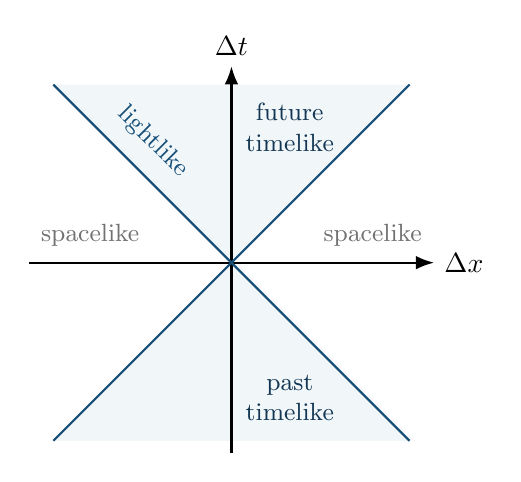
\begin{tikzpicture}[scale=0.78,>=Latex]
  \fill[paleBlue] (0,0)--(-2.9,2.9)--(2.9,2.9)--cycle;
  \fill[paleBlue] (0,0)--(-2.9,-2.9)--(2.9,-2.9)--cycle;
  \draw[->,thick] (-3.3,0)--(3.3,0) node[right] {\(\Delta x\)};
  \draw[->,thick] (0,-3.1)--(0,3.2) node[above] {\(\Delta t\)};
  \draw[blue,thick] (-2.9,-2.9)--(2.9,2.9);
  \draw[blue,thick] (-2.9,2.9)--(2.9,-2.9)
    node[pos=0.22,sloped,above=3pt,font=\small] {lightlike};
  \node[navy,align=center,font=\small] at (0.95,2.2) {future\\timelike};
  \node[navy,align=center,font=\small] at (0.95,-2.2) {past\\timelike};
  \node[ink!75,font=\small] at (2.3,0.45) {spacelike};
  \node[ink!75,font=\small] at (-2.3,0.45) {spacelike};
\end{tikzpicture}

{\small A \(1+1\)-dimensional section with
\(\Delta y=\Delta z=0\) and \(c=1\).}
\end{center}

\begin{theorem}{Canonical forms of a displacement}{canonical-displacement}
After a spatial rotation and a proper orthochronous Lorentz boost, a nonzero
displacement has one of the following canonical forms.
\begin{enumerate}
  \item If \(d^2>0\), there is a frame in which
  \[
    d^\mu=(\pm\sqrt{d^2},0,0,0),
  \]
  the sign is positive for a future-directed displacement and negative for a
  past-directed one.
  \item If \(d^2=0\) and \(d^\mu\ne0\), there is no frame in which the events
  are simultaneous or colocated, and a suitable orientation gives
  \[
    d^\mu=(\lambda,\lambda,0,0),\qquad \lambda\ne0,
  \]
  with the time orientation fixing the sign of \(\lambda\). Its magnitude
  can be changed by a boost and is not an invariant.
  \item If \(d^2<0\), there is a frame in which
  \[
    d^\mu=(0,\sqrt{-d^2},0,0).
  \]
\end{enumerate}
\end{theorem}

The three signs correspond to three distinct causal possibilities. Timelike
separated events can occur at the same place in some inertial frame. Spacelike
separated events can occur at the same time in some inertial frame, and their
temporal order can be reversed by changing frames. A nonzero null displacement
admits neither a common-place frame nor a simultaneous frame.

\begin{precision}[Time ordering]
For timelike or distinct lightlike separated events, their temporal order is
the same in every orthochronous inertial frame. Spatial reflection does not
alter this conclusion, whereas time reversal does. For spacelike separated
events, neither temporal ordering is shared by all such frames.
\end{precision}

\begin{studentwork}[height=8.0cm]{proof}
Prove Theorem~\ref{thm:canonical-displacement}.
\end{studentwork}

\subsection{Intervals and clock readings}

For a timelike separation, the canonical frame contains an inertial clock
that passes through both events. The elapsed time on that clock is
\(\sqrt{\Delta s^2}/c\). The qualification \emph{inertial} matters because
the reading of a clock on an accelerated path depends on the path, not just
its endpoints.

\begin{definition}{Proper time}{proper-time}
Along a future-directed timelike worldline, the \emph{proper time} \(\tau\)
is the time measured by an ideal clock following that worldline. Its
infinitesimal increment is
\[
  \dd\tau=\frac{1}{c}\sqrt{g_{\mu\nu}\dd x^\mu\dd x^\nu}
  =\sqrt{1-\frac{\lVert\vect u\rVert^2}{c^2}}\,\dd t,
  \qquad \vect u=\frac{\dd\vect x}{\dd t},
\]
where \(x^0=ct\), \(\dd t>0\), and \(\lVert\vect u\rVert<c\).
The elapsed proper time is the integral of this expression along the path.
\end{definition}

For spacelike separated events, \(\sqrt{-\Delta s^2}\) is their spatial
separation in a frame in which they are simultaneous. A nonzero null
worldline has no inertial rest frame. Thus a null interval must not be
interpreted as the reading of a clock in a photon's rest frame.

\section{Four-momentum and invariant mass}
\slideref{14}

Momentum and energy combine into one Lorentz-covariant object. In natural
units, the energy-momentum four-vector is
\[
  p^\mu=(E,\vect{p}).
\]
For a massive particle, a rest frame exists in which
\(\vect p=\vect{0}\). The rest mass \(m\) is defined by the rest-frame energy
\(E_{\mathrm{rest}}=m\) in natural units. Since \(p^2=p\cdot p\) is invariant,
\[
\boxed{p^2=E^2-\lVert\vect{p}\rVert^2=m^2.}
\]
Restoring \(c\) gives
\[
\boxed{E^2=\lVert\vect{p}\rVert^2c^2+m^2c^4.}
\]

\begin{precision}[Massless particles]
A massless particle has no rest frame. Its four-momentum is null, so
\[
  p^2=0,\qquad E=c\lVert\vect{p}\rVert
\]
for a positive-energy particle. The rest-frame argument applies only when
\(m>0\). With \(c\) explicit, the invariant relation is \(p^2=m^2c^2\).
In units \(c=1\), it is \(p^2=m^2\), including the massless case.
\end{precision}

\begin{studentwork}[height=6.5cm]{derivation}
Derive the energy-momentum relation and restore the factors of \(c\).
\end{studentwork}

For an isolated collision, four-momentum conservation states
\[
  P^\mu_{\mathrm{in}}=\sum_{i\in\mathrm{in}}p_i^\mu
  =\sum_{j\in\mathrm{out}}p_j^\mu=P^\mu_{\mathrm{out}}.
\]
Call this common total four-momentum \(P\). Conservation compares its value
before and after the collision, whereas Lorentz invariance compares \(P^2\)
between frames. These are different statements. In units \(c=1\), the
Mandelstam variable \(s\) for two incoming particles is
\[
  s=(p_1+p_2)^2.
\]
If \(P\) is timelike and future-directed, a center-of-momentum frame exists.
There \(\vect P=\vect0\), so \(\sqrt{s}\) is the total center-of-momentum
energy. The symbol \(s\) here is a momentum invariant, not the spacetime
interval \(\Delta s^2\).

\begin{studentwork}[height=5.8cm]{calculation}
Expand \(s=(p_1+p_2)^2\) in terms of \(m_1,m_2\), and \(p_1\cdot p_2\).
\end{studentwork}

\section{Lorentz and Poincar\'e transformations}
\label{sec:lorentz-poincare}
\slideref{15}

The invariant interval now determines the allowed transformations between
inertial coordinate systems. Translations alter the chosen spacetime origin,
while the linear part must preserve the Minkowski metric.

\begin{definition}{Lorentz transformation}{lorentz-transformation}
A linear map \(\Lambda:\R^4\to\R^4\) is a \emph{Lorentz transformation} if it
preserves the Minkowski scalar product. Thus
\[
  (\Lambda p)\cdot(\Lambda q)=p\cdot q
  \qquad\text{for all }p,q.
\]
In matrix notation this is equivalent to
\[
\boxed{\Lambda^{\transpose}g\Lambda=g.}
\]
\end{definition}

All Lorentz transformations form the group \(O(1,3)\), where \(1,3\) count
the positive and negative signs of the metric. The Lorentz condition implies
\(\det\Lambda=\pm1\) and \(|\Lambda^0{}_0|\geq1\). These two sign choices
distinguish four connected components. Here a connected component is a
maximal family within which matrices can be joined by continuous paths that
remain Lorentz transformations.

The component containing the identity is the \emph{proper orthochronous}
Lorentz group \(SO^+(1,3)\), characterized by
\[
  \det\Lambda=+1,\qquad \Lambda^0{}_0\geq1.
\]
It contains ordinary spatial rotations and boosts. Time reversal and spatial
reflection are also in \(O(1,3)\), but not in this component. The adjective
\emph{proper} by itself does not exclude time reversal combined with spatial
reflection.

\begin{definition}{Poincar\'e transformation}{poincare-transformation}
An affine spacetime transformation
\[
  x'^\mu=\Lambda^\mu{}_\nu x^\nu+a^\mu
\]
with Lorentz matrix \(\Lambda\) is a \emph{Poincar\'e transformation}. The
special case \(a^\mu=0\) is a homogeneous Lorentz transformation.
\end{definition}

\begin{precision}
The expression \emph{inhomogeneous Lorentz transformation} is sometimes used
for \((\Lambda,a)\). The standard name for the complete symmetry group is the
Poincar\'e group. Translations do not change event displacements, so preservation
of intervals reduces to the Lorentz condition on \(\Lambda\).
\end{precision}

The Lorentz group has six continuous parameters near the identity, consisting
of three rotation parameters and three boost parameters. Adding four
translations makes the Poincar\'e group ten-dimensional.

\begin{studentwork}[height=6.0cm]{derivation}
Derive the matrix condition for a Lorentz transformation and determine the
number of independent infinitesimal parameters.
\end{studentwork}

\section{The standard boost}
\slideref{16}

A proper orthochronous Lorentz transformation can be built from rotations and
boosts. The other components also require a discrete reflection or time
reversal. To isolate the simplest boost, let \(O'\) move with signed physical
velocity \(V\) along the \(x\)-axis relative to \(O\). Choose coincident origins at
\(t=t'=0\) and parallel spatial axes. Symmetry then gives \(y'=y\) and
\(z'=z\), so only \(x^0=t\) and \(x^1=x\) mix in units \(c=1\).

The full four-dimensional matrix, denoted by \(\Lambda(V)\), has block form
\[
\Lambda(V)=
\begin{pmatrix}
  \Lambda^0{}_0 & \Lambda^0{}_1 & 0 & 0\\
  \Lambda^1{}_0 & \Lambda^1{}_1 & 0 & 0\\
  0&0&1&0\\
  0&0&0&1
\end{pmatrix}.
\]
The unchanged transverse coordinates already preserve their contribution
\(- (\Delta y)^2- (\Delta z)^2\) to the interval. The metric restricted to the
\((t,x)\)-plane is represented by
\[
  g_{(1+1)}
  :=
  \begin{pmatrix}
    1&0\\
    0&-1
  \end{pmatrix}.
\]
The notation \(1+1\) indicates one time and one spatial dimension. The
remaining problem is therefore to find its \(2\times2\) boost block \(L\),
which must preserve this restricted metric. Thus \(\Lambda(V)=\operatorname{diag}(L,\id_2)\). Here \(L\) and \(\Lambda\) denote the block and the full matrix, respectively.

\begin{studentwork}[height=6.8cm]{derivation}
Obtain the independent conditions on the four entries of the boost block.
\end{studentwork}

\section{Determining the boost matrix}
\slideref{17}

Write the unknown \(1+1\)-dimensional block as
\[
  L=
  \begin{pmatrix}\ell_{00}&\ell_{01}\\\ell_{10}&\ell_{11}\end{pmatrix}.
\]
The subscripts on \(\ell_{ab}\) label matrix positions only. They are not
lowered Lorentz indices.
The Lorentz condition is
\[
  L^{\transpose}g_{(1+1)}L=g_{(1+1)}.
\]

\begin{theorem}{Boost connected to the identity}{boost-rapidity}
Every real \(2\times2\) matrix satisfying
\(L^{\transpose}g_{(1+1)}L=g_{(1+1)}\) in the component containing the
identity can be written uniquely as
\[
\boxed{
L(\eta)=
\begin{pmatrix}
  \cosh\eta&-\sinh\eta\\
  -\sinh\eta&\cosh\eta
\end{pmatrix},
}
\]
where \(\eta\in\R\) is the rapidity.
\end{theorem}

\begin{precision}
The group \(O(1,1)\) has four disconnected components. The standard boosts
\(L(\eta)\) form the component containing the identity because
\(L(0)=\id_2\) and varying \(\eta\) continuously connects each boost to
\(\id_2\).

The other components are obtained by combining \(L(\eta)\) with spatial
reflection \(P=\operatorname{diag}(1,-1)\), time reversal
\(T=\operatorname{diag}(-1,1)\), or both. They therefore have the forms
\[
  PL(\eta),\qquad TL(\eta),\qquad PTL(\eta).
\]
In these products the boost acts first. The matrices \(P\) and \(T\) then
reverse the resulting spatial and temporal coordinates, respectively.
The signs of the matrix entries are constrained by the Lorentz condition and
cannot be chosen independently.
\end{precision}

\begin{studentwork}[height=11.0cm]{proof}
Prove Theorem~\ref{thm:boost-rapidity}.
\end{studentwork}

\section{Rapidity and relative velocity}
\slideref{18}

The rapidity parameter acquires physical meaning by following the primed
origin. Let \(A\) and \(B\) be two events on its worldline, with \(A\) chosen
as the common origin. The displacement from \(A\) to \(B\) has components
\[
  \Delta x^\mu=(\Delta t,V\Delta t,0,0)
  \quad\text{in }O,
  \qquad
  \Delta x'^\mu=(\Delta t',0,0,0)
  \quad\text{in }O'.
\]
Applying the boost of Theorem~\ref{thm:boost-rapidity} gives
\[
\begin{pmatrix}\Delta t'\\0\end{pmatrix}
=
\begin{pmatrix}
  \cosh\eta&-\sinh\eta\\
  -\sinh\eta&\cosh\eta
\end{pmatrix}
\begin{pmatrix}\Delta t\\V\Delta t\end{pmatrix}.
\]

\begin{proposition}{Velocity, rapidity, and the Lorentz factor}{velocity-rapidity}
For a standard boost with \(|V|<c\), define \(\beta=V/c\). Then
\[
  \beta=\tanh\eta,\qquad
  \gamma=\frac{1}{\sqrt{1-\beta^2}}=\cosh\eta,\qquad
  \gamma\beta=\sinh\eta.
\]
In units \(c=1\), \(V\) and \(\beta\) have the same numerical value.
With \(c\) displayed explicitly, the standard boost is
\[
\boxed{
\begin{aligned}
  ct'&=\gamma(ct-\beta x),\\
  x'&=\gamma(x-\beta ct),\\
  y'&=y,\qquad z'=z.
\end{aligned}}
\]
\end{proposition}

\begin{studentwork}[height=9.5cm]{derivation}
Derive Proposition~\ref{prop:velocity-rapidity}.
\end{studentwork}

The nonrelativistic limit is controlled by the dimensionless velocity
\(\beta=V/c\). When \(|\beta|\ll1\),
\[
  \eta=\operatorname{artanh}\beta=\beta+\order{\beta^3},
  \qquad
  \gamma=1+\frac12\beta^2+\order{\beta^4}.
\]
Equivalently, the boost block has the expansion
\[
  \begin{pmatrix}ct'\\x'\end{pmatrix}
  =\left[
    \id_2-\beta\begin{pmatrix}0&1\\1&0\end{pmatrix}
    +\frac{\beta^2}{2}\id_2+\order{\beta^3}
  \right]
  \begin{pmatrix}ct\\x\end{pmatrix}.
\]
Keeping the terms linear in \(\beta\) gives
\(x'\simeq x-Vt\) and \(t'\simeq t-Vx/c^2\). The Galilean limit is more
precisely obtained by letting \(c\to\infty\) at fixed \(V,x,t\). Then
\(\gamma\to1\), \(t'\to t\), and \(x'\to x-Vt\).

\begin{proposition}{Composition of collinear boosts}{rapidity-addition}
For collinear boosts,
\[
  L(\eta_2)L(\eta_1)=L(\eta_1+\eta_2).
\]
Velocities do not add linearly, but rapidities do.
If \(V_1\) is the velocity of \(O'\) in \(O\) and \(V_2\) is the velocity
of \(O''\) in \(O'\), with parallel axes, the velocity of \(O''\) in \(O\)
is
\[
  V_{\mathrm{tot}}=\frac{V_1+V_2}{1+V_1V_2/c^2}.
\]
\end{proposition}

\begin{studentwork}[height=7.0cm]{proof}
Prove both the rapidity and velocity composition laws in
Proposition~\ref{prop:rapidity-addition}.
\end{studentwork}

\section{Four-vectors and covectors}
\slideref{19}

A spacetime displacement is the difference of two events in the affine
spacetime \(\mathcal M\). Because translations cancel, its components transform
homogeneously according to
\[
  \Delta x'^\mu=\Lambda^\mu{}_\nu\Delta x^\nu.
\]
A \emph{four-vector} \(V\) has components obeying the same linear law,
\(V'^\mu=\Lambda^\mu{}_\nu V^\nu\), although it need not physically be a
displacement. Four-momentum, for example, has units of momentum. A
\emph{covector} is a linear functional on four-vectors. If its components are
\(W_\mu\), the pairing \(W_\mu V^\mu\) is a scalar and must be independent of
the inertial basis.

\begin{proposition}{Covector transformation law}{covector-law}
If \(V'^\mu=\Lambda^\mu{}_\nu V^\nu\), scalar invariance requires
\[
\boxed{
  W'_\mu=(\Lambda^{-1})^\nu{}_\mu W_\nu.
}
\]
\end{proposition}

\begin{studentwork}[height=7.0cm]{proof}
Prove Proposition~\ref{prop:covector-law}.
\end{studentwork}

For the standard boost,
\[
  L(\eta)^{-1}=L(-\eta),
  \qquad
  \Lambda(V)^{-1}=\Lambda(-V).
\]
This has a direct physical meaning. The velocity of \(O\) as measured in
\(O'\) is the negative of the velocity of \(O'\) as measured in \(O\).

\begin{studentwork}[height=5.3cm]{verification}
Verify \(L(\eta)^{-1}=L(-\eta)\).
\end{studentwork}

\section{The metric and index operations}
\slideref{20}

The metric not only produces invariant scalars. It also identifies vectors with
covectors. In the standard inertial basis, the metric and inverse metric have
components
\[
  (g_{\mu\nu})=\operatorname{diag}(1,-1,-1,-1),
  \qquad
  (g^{\mu\nu})=\operatorname{diag}(1,-1,-1,-1),
\]
and satisfy
\[
  g^{\mu\nu}g_{\nu\rho}=\delta^\mu{}_\rho.
\]
They lower and raise indices according to
\[
  V_\mu=g_{\mu\nu}V^\nu,
  \qquad
  V^\mu=g^{\mu\nu}V_\nu.
\]
Thus, if \(V^\mu=(V^0,V^1,V^2,V^3)\), then
\[
  V_\mu=(V^0,-V^1,-V^2,-V^3).
\]

\begin{proposition}{Inverse of a Lorentz matrix}{lorentz-inverse}
The Lorentz condition implies
\[
\boxed{
  \Lambda^{-1}=g^{-1}\Lambda^{\transpose}g.
}
\]
In the standard inertial basis, \(g^{-1}=g\), so this is also
\(\Lambda^{-1}=g\Lambda^{\transpose}g\). In components, define
\[
  \Lambda_\mu{}^\nu
  :=g_{\mu\alpha}\Lambda^\alpha{}_\beta g^{\beta\nu}.
\]
Then
\[
  (\Lambda^{-1})^\mu{}_\nu=\Lambda_\nu{}^\mu.
\]
\end{proposition}

\begin{studentwork}[height=7.8cm]{proof}
Prove Proposition~\ref{prop:lorentz-inverse}.
\end{studentwork}

Combining the metric with the vector transformation gives
\[
  V'_\mu
  =(\Lambda^{-1})^\nu{}_\mu V_\nu
  =\Lambda_\mu{}^\nu V_\nu.
\]
The upper-index and lower-index formulas therefore encode the vector and dual
representations of the Lorentz group.
In matrix notation, if the components of both objects are stored as columns,
the vector column transforms with \(\Lambda\), whereas the covector column
transforms with \((\Lambda^{-1})^{\transpose}\). Writing a covector as a row
instead gives right multiplication by \(\Lambda^{-1}\).

\begin{studentwork}[height=5.8cm]{derivation}
Derive the lower-index transformation law.
\end{studentwork}

\section{Lorentz transformations of fields}
\slideref{21}

A field assigns a quantity to every event in a region of spacetime. The type
of that quantity determines the field's transformation law. The fields below
are taken to be smooth, so that derivatives can be formed when needed. No
field equation is assumed.

\subsection{One event, two coordinate descriptions}

Let \(X\in\mathcal M\) be one event. Inertial frames \(O\) and \(O'\) assign
it coordinates \(x=\chi_O(X)\) and \(x'=\chi_{O'}(X)\), related by
\[
  x'^\mu=\Lambda^\mu{}_\nu x^\nu+a^\mu.
\]
The argument displayed in a component function is therefore a coordinate label
for \(X\), not a second event.

\begin{definition}{Scalar field transformation}{scalar-field}
A geometric scalar field is a map \(\Phi:\mathcal M\to\R\). Its coordinate
representatives \(\phi=\Phi\circ\chi_O^{-1}\) and
\(\phi'=\Phi\circ\chi_{O'}^{-1}\) satisfy
\[
\boxed{\phi'(x')=\phi(x).}
\]
\end{definition}

\begin{definition}{Vector and covector field transformations}{vector-field}
A vector field assigns a spacetime vector to each event, while a covector field
assigns a dual vector. Their components at the same event satisfy
\[
  A'^\mu(x')=\Lambda^\mu{}_\nu A^\nu(x),
  \qquad
  W'_\mu(x')=(\Lambda^{-1})^\nu{}_\mu W_\nu(x).
\]
Here \(A\) and \(W\) can be independent fields. If \(W_\mu=g_{\mu\nu}A^\nu\),
the covector field is the metric dual of \(A\).
\end{definition}

\begin{theorem}{General tensor field transformation}{tensor-field-law}
For a tensor field of type \((r,s)\),
\[
\begin{aligned}
T'^{\mu_1\cdots\mu_r}{}_{\nu_1\cdots\nu_s}(x')
={}&
\Lambda^{\mu_1}{}_{\alpha_1}\cdots
\Lambda^{\mu_r}{}_{\alpha_r}\\
&\times
(\Lambda^{-1})^{\beta_1}{}_{\nu_1}\cdots
(\Lambda^{-1})^{\beta_s}{}_{\nu_s}
T^{\alpha_1\cdots\alpha_r}{}_{\beta_1\cdots\beta_s}(x).
\end{aligned}
\]
\end{theorem}

\begin{precision}[Upper and lower indices]
With the convention
\[
  V'^\mu=\Lambda^\mu{}_\nu V^\nu,
\]
every upper index transforms with a factor of \(\Lambda\). A lower index
transforms with the inverse matrix,
\[
  \omega'_\mu
  =(\Lambda^{-1})^\nu{}_\mu\omega_\nu.
\]
This opposite transformation ensures that the contraction of a covector and a
vector remains unchanged,
\[
  \omega'_\mu V'^\mu=\omega_\mu V^\mu.
\]

Each index of a tensor transforms separately. For example,
\[
  T'^\mu{}_\nu
  =
  \Lambda^\mu{}_\alpha
  (\Lambda^{-1})^\beta{}_\nu
  T^\alpha{}_\beta.
\]
The notation \(\Lambda_\mu{}^\nu=(\Lambda^{-1})^\nu{}_\mu\) is defined by
raising and lowering the matrix indices with the metric. If both input and
output covector components are arranged as columns, the corresponding matrix
is \((\Lambda^{-1})^{\transpose}\), not \(\Lambda\). Index positions and
index order must therefore be respected.
\end{precision}

\begin{studentwork}[height=9.5cm]{derivation}
Derive Theorem~\ref{thm:tensor-field-law}.
\end{studentwork}

\subsection{Passive and active viewpoints}

The equations above use the passive viewpoint. The geometric event is fixed,
while its coordinates and the components used to describe field values change.
Write the coordinate change as \(x'=F(x)=\Lambda x+a\). Solving for the old
coordinates gives \(x=F^{-1}(x')\). Thus the scalar-field law can also be
written as an equality of functions,
\[
  \phi'(z)=\phi\bigl(F^{-1}(z)\bigr)
  =\phi\!\left(\Lambda^{-1}(z-a)\right),
\]
where \(z\) is an arbitrary numerical coordinate tuple. The inverse appears
because the value expressed in new coordinates must be found at the matching
old coordinates. This is still the same field, expressed in two charts.

For an \emph{active} transformation, keep one coordinate chart fixed and move
the field configuration by the spacetime map represented by \(F\). Denote
the resulting scalar field by \(\phi_F\). A value originally at \(x\) is
carried to \(F(x)\), so
\[
  \phi_F\bigl(F(x)\bigr)=\phi(x),
  \qquad
  \phi_F(x)=\phi\bigl(F^{-1}(x)\bigr).
\]
The algebraic form is the same, but the interpretation differs. A passive
transformation relabels a fixed configuration. An active transformation
changes the configuration in a fixed chart. For example, an active spatial
translation by \(a\) sends \(\phi(x)\) to \(\phi(x-a)\), moving its profile
by \(+a\).

For a vector field the active transformation also changes the components,
\[
  A_F^\mu(x)
  =\Lambda^\mu{}_\nu A^\nu\bigl(F^{-1}(x)\bigr).
\]
The inverse in the argument and the factor multiplying the field value play
different roles. Whether such a transformation maps solutions of a field
equation to solutions is a question about that equation, not just its
notation.

\begin{studentwork}[height=10.0cm]{derivation}
Derive the same-coordinate transformation law for a scalar field.
\end{studentwork}

\end{document}